\documentclass[11pt]{article}

\usepackage[letterpaper,left=1in,right=1in,top=1in,bottom=1in]{geometry}
\usepackage{float}
\usepackage[T1]{fontenc}
\usepackage[utf8]{inputenc}

\usepackage{lmodern}
\usepackage{amssymb,amsmath}

\setcounter{secnumdepth}{0}

%\usepackage[vlined]{algorithm2e}
\usepackage{algorithm,algorithmic}
\usepackage{paralist}
\usepackage{tikz}
\usepackage{xcolor,colortbl}
\usepackage{multicol}

\usepackage{listings}

\begin{document}
\lstset{
language=Python,
basicstyle=\ttfamily\scriptsize,        % the size of the fonts that are used for the code
frame=single,                    % adds a frame around the code
keepspaces=true,                 % keeps spaces in text, useful for keeping indentation of code (possibly needs columns=flexible)
keywordstyle=\color{blue},
commentstyle=\color{gray}
}
\setlength{\parindent}{0in}
\addtolength{\parskip}{0.1cm}
\setlength{\fboxrule}{.5mm}\setlength{\fboxsep}{1.2mm}
\newlength{\boxlength}\setlength{\boxlength}{\textwidth}
\addtolength{\boxlength}{-4mm}

\begin{center}\framebox{\parbox{\boxlength}{{\bf
CS 4740, Spring 2014 \hfill Project 2 Report}\\
Anthony Chen (apc52)\\ 
James Feher (jkf49)\\ 
Matthew Oey (mso32)
}}
\end{center}

\section{Approach}
\subsection{Supervised WSD}
\subsubsection{Parsing Input Data and Data Structures}

To handle the input data, we used a word object. For every word $w_i$, the object holds the string value for the word and part of speech, as well as a map of senses to the cooresponding context lists. Context lists are the set of contexts that in which that word is used with that sense. For each context, we use NLTK to tokenize the input and then we separate the context into four parts: the sentences prior to the sentence containing $w_i$, the words in the sentence that come before the word $w_i$, the words in the sentence that come after the word $w_i$, and the sentences after to the sentence containing $w_i$. The input data is parsed by having a global map containing mappings of word strings to word objects. 

\begin{lstlisting}
#wordmap is a mapping of word strings to word objects
def parse_train_data(filename):
    word_map = {}
    with open(filename) as f:
        for line in f:
            parts = re.split(' \| ', line)
            splitByPeriod = re.split('\.', parts[0])
            word = splitByPeriod[0]
            pos = splitByPeriod[1]
            sense = parts[1]
            context = parts[2]

            #Create word map
            if not word in word_map:
                word_map[word] = Word(word, pos)
            word_map[word].add_context(sense, context)

    return word_map
\end{lstlisting}

\subsubsection{Preprocessing}
As part of our preprocessing stage, we need to know the number of examples we have for each sense for each word. The following simple function takes as input the word map created above and iterates across each word object, calculating the sense count, to output a mapping of words to senses to the number of examples in our training set.

\begin{lstlisting}
def get_sense_count(word_map):
    word_to_sense_to_count_map = {}
    for word_object in word_map.values():
        sense_to_count_map = {}
        for sense, context_list in word_object.sense_id_map.items():
            sense_to_count_map[sense] = float(len(context_list))
        word_to_sense_to_count_map[word_object.word] = sense_to_count_map
    return word_to_sense_to_count_map
\end{lstlisting}

The other part of our preprocessing is that we need to know how many target words there are in the context for each sense of each word. This function, similar to the one above, calculates those scores by iterating across each word object sense and calculates the number of examples that contain a certain target word and from that calculates the probability that a target word has to a particular sense.

\begin{lstlisting}
def get_target_probability(word_map):
    word_to_sense_to_target_prob_map = {}
    for word_object in word_map.values():
        sense_to_target_count_map = {}
        for sense, context_list in word_object.sense_id_map.items():
            count = 1
            if sense not in sense_to_target_count_map:
                sense_to_target_count_map[sense] = {}
            for context in context_list:
                count +=1
                target = context.target
                if target in sense_to_target_count_map[sense]:
                    sense_to_target_count_map[sense][target] += 1
                else:
                    sense_to_target_count_map[sense][target] = 1
            for target in sense_to_target_count_map[sense]:
                sense_to_target_count_map[sense][target] /= float(count + 1)
            sense_to_target_count_map[sense]['<UNK>'] = 1 / float(count + 1)
        word_to_sense_to_target_prob_map[word_object.word] = sense_to_target_count_map
    return word_to_sense_to_target_prob_map
\end{lstlisting}

To keep track of our features, we decided to use a unigram model. Using the techniques we learned from Project 1, we created a unigram for each word sense using the training data. This unigram would hold the probability that each of our features would appear in the context. To create this, we iterated over each word and sense and for each context we iterated across the token list to find the count of each word. We also decided to apply Good-Turing smoothing and use our methods for handling unknown words from the previous project. \\ 

\subsubsection{Classifying data}
In supervised training, we used three main features for classification. The first two features are unigrams within plus or minus $k$ words from the target word. Early in our testing we tried different values of $k$ and found that the value that consistently gave us the best scores was at $k=5$. We used this value of $k$ both to train our model by only considering $k$ words to the left, and $k$ words to the right when constructing the unigram models. Again, in our testing, we found that splitting previous context and after context into separate features improved the performance of our classifier. Our third feature is the target word. For example, on lines 98 and 104(and other lines), you can see this is for training the word allow.v.2. Both of these words have the same sense and they also have the exact same target word: allowed, rather than allow. This made think to try adding the target word as a feature and improved our accuracy. Though not a feature, the last thing we added to our classifier is the ability to skip words common words by using the nltk stopwords list. The results with these features are discussed below. 

To classify each word $w_i$ in our validation set, we iterated across each context in the set of unclassified words. For each of the possible senses for that word, we then used the unigram models and target word probabilities associated with that sense to find the probability of each feature in the context. We then used this to calculate the probability that $w_i$ has sense $s_i$ given the features in the context using the naive bayes algorithm. We keep track of our best probabilty and we output the sense assciated with that probability as our guess.

\begin{lstlisting}
def score_validation_set(unclassified_words, unigram_model, word_map, outputFile):
    word_to_sense_probability_map = get_sense_probability(word_map)
    target_word_prob_map = get_target_probability(word_map)
    text_file = open("output.txt", "w")
    for word_object in unclassified_words:
        bestSense = 0
        bestProbability = 0
        for sense in unigram_model[word_object.word]:
            unigram_probability = unigram_model[word_object.word][sense]
            probability = word_to_sense_probability_map[word_object.word][sense]
            context = word_object.sense_id_map[0][0]
            prev, after = context.prev_context, context.after_context
            for i in range(len(prev)-NUM_NGRAMS_OBSERVED-1, len(prev)-1):
                unigram_probability_left = unigram_probability['left']
                if i < 0 :
                    #probability *= unigram_probability_left['<UNK>']
                    continue
                token = lmtzr.lemmatize(prev[i])
                if token in unigram_probability_left:
                    probability *= unigram_probability_left[token]
                else:
                    probability *= unigram_probability_left['<UNK>']
            for i in range(len(after)-NUM_NGRAMS_OBSERVED-1, len(after)-1):
                unigram_probability_right = unigram_probability['right']
                if i < 0 :
                    #probability *= unigram_probability_right['<UNK>']
                    continue
                token = lmtzr.lemmatize(after[i])
                if token in unigram_probability_right:
                    probability *= unigram_probability_right[token]
                else:
                    probability *= unigram_probability_right['<UNK>']
            if context.target in target_word_prob_map[word_object.word][sense]:
                probability *= target_word_prob_map[word_object.word][sense][context.target]
            else:
                probability *= target_word_prob_map[word_object.word][sense]['<UNK>']
            if probability > bestProbability:
                bestProbability = probability
                bestSense = sense
        text_file.write(bestSense + "\n")
    text_file.close()
\end{lstlisting}		
	

\subsection{Dictionary WSD}
\subsubsection{Parsing and Data Structures}
The dictionary datafile parser generates a Dictionary object, which is a Python dictionary that holds Word objects. Word objects were also used in the parsing of the supervised WSD datasets. The Word object was used in both WSD methods because there were overlaps in the test dataset parsing methods. The Word object was augmented, however, to contain a dictionary of senses. For every word, the dictionary dataset parser created its constituent senses as Sense objects. Figure~\ref{sense} shows the data structure. The gloss and example sentences were tokenized using NLTK.

\begin{figure}[ht]
\begin{lstlisting}
class Sense:
    def __init__(self,id,wordnet_ids,gloss,examples):
        self.id = id # The dictionary dataset sense of a word
        self.wordnet_ids = wordnet_ids # List of characters
        self.gloss = gloss # List of tokens (lemmatized or not)
        self.examples = examples # List of lists of tokens (lemmatized or not)
\end{lstlisting}
\caption{Sense object for dictionary WSD}
\label{sense}
\end{figure}

\subsubsection{Word-sense Disambiguation}
The WSD algorithm is similar to Lesk's algorithm. First, the method parses the test dataset using parse\_test\_data(). Then, for every word (also the test case) in the test dataset, features are selected from the word's context. These features are passed, along with the target word, to the method find\_best\_sense(). The method find\_best\_sense() constructs a general features context, which is comprised of a signature from each feature. A signature is a list of lists of tokens, representing the tokenized definition and examples of a feature. A signature is also constructed for every sense of the target word. An overlap score is then calculated between each target word sense signature and the word's features context to determine which sense is the best. 

During the overlap score calculation, shown in Figure~\ref{overlap}, the target sense signature is compared to every feature signature in the features context to determine if overlaps of two or more tokens appear. An overlap of two or more tokens is considered a \textit{sequence}, which contributes to the sense's overall score. Longer overlap sequences are weighted heavier, according to the formula $score = \frac{n(n+1)}{2} - 1$, where $n$ is the length of the overlap. The overlap sequences are also weighted according to the importance of the constituent token. Importance of a token is approximated by the token's inverse document frequency. The sum of the IDF scores of each token represent the sequence's final score.

\begin{figure}[ht]
\begin{lstlisting}
def calculate_overlap_score(idf_map, target_token_list, context_token_list):
    score = 0.0
    if len(context_token_list) == 0:
        return score
    for i in range(len(target_token_list)):
        original_i = i
        for j in range(len(context_token_list)):
            i = original_i
            matched = []
            while i < len(target_token_list) and j < len(context_token_list):
                if target_token_list[i] == context_token_list[j]:
                    matched.append(target_token_list[i])
                    i += 1
                    j += 1
                else:
                    break
            if len(matched) >= 2:
                acc = 0.0
                for match in matched:
                    acc += idf_map[match]
                weight = acc / len(matched)
                score += weight
    return score
\end{lstlisting}
\caption{Overlap score calculation method}
\label{overlap}
\end{figure}

\subsubsection{Feature Selection}
Feature selection from a target word's context also considered importance via a token's inverse document frequency. Every token in a target word's context was assigned a weight that was their IDF. A threshold was set that filtered the context into a set of features. The threshold was set experimentally to the value of $6.0$.

\subsubsection{Lemmatization}
We included an optional lemmatization step in both the parsing of the dictionary dataset and the disambiguation. Tokens from the sense gloss and example sentences are lemmatized, as well as the features provided to word\_sense\_disambiguation() and the feature synset definition and example sentences. The reasoning in lemmatizing tokens was to reduce false negatives in calculating overlaps, due to morphological variations in words.

\section{Software}
\subsection{Supervised WSD}
For Supervised WSD we used NLTK 

\subsection{Dictionary WSD}
The Python Standard Library ElementTree XML API was utilized to parse the dictionary XML file and generate a hierarchical set of data structures representing the dictionary datafile contents. Libraries from the Natural Language Toolkit (NLTK) were also used extensively in the parsing of the dictionary dataset and in the disambiguation process. Specifically, the word tokenizer, part of speech tagger, and lemmatizer were used.

\section{Results}
\subsection{Supervised WSD}
\begin{table}[H]
    \begin{tabular}{|l|l|}
    \hline
    Features                                                                        & ~       \\ \hline
    target word probability + unigram(window size 5) + stoplist                     & 0.81266 \\ \hline
    target word probability + unigram(window size 5)                                & 0.80704 \\ \hline
    target word probability + unigram(window size 5) no validation set              & 0.80449 \\ \hline
    target word probability + unigram(window size 5) with synsets no validation set & 0.80424 \\ \hline
    target word probability + unigram(window size 10) no validation set             & 0.80092 \\ \hline
    unigram(window size 10)                                                         & 0.79888 \\ \hline
    unigram(window size 5)                                                          & 0.79735 \\ \hline
    most common sense baseline                                                      & 0.78076 \\ \hline
    random baseline                                                                 & 0.33     \\ \hline
    \end{tabular}
\end{table}

Here we present the results of a few of our trials sorted in decreasing order of efficiency based on the kaggle test set. We have two baselines which were guessing a random sense which scored approximately .33. Surprisingly, just guessing the most common sense is enough to get a score of .78076. We then created our naive bayes classifier by adding on features incrementally. 

\subsubsection{Feature Selection}
\begin{center}
\begin{table}
    \begin{tabular}{|l|l|}
    \hline
    Submission                          & Score   \\ \hline
    Used a stop list to select features & 0.81266 \\
    Used features with idf > 2.0        & 0.80704 \\
    Used all features                   & 0.80704 \\
    Most common senses(baseline)        & 0.78076 \\ \hline
    \end{tabular}
\end{table}
\end{center}

\subsubsection{Extension 4}
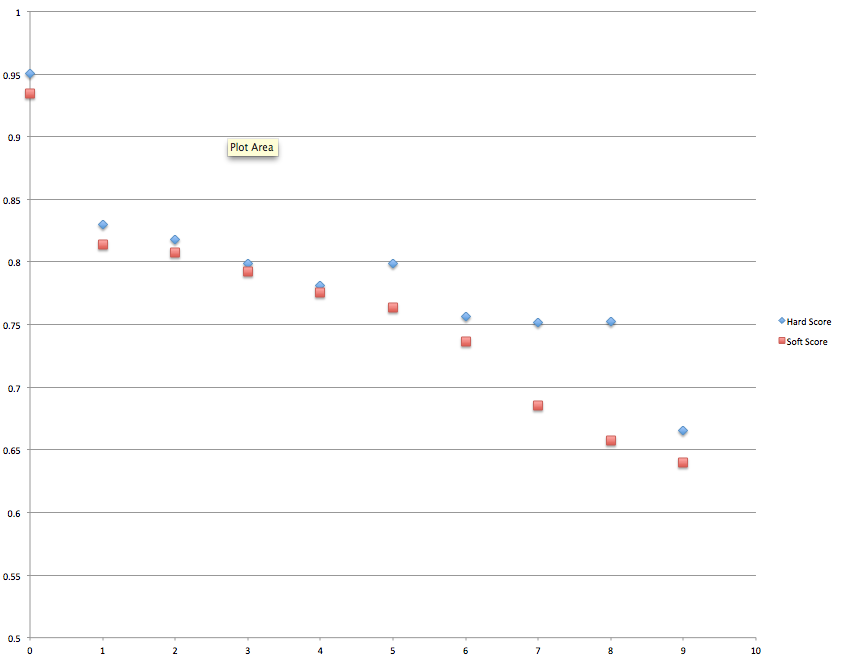
\includegraphics[width = 4in]{data_plot.png}

\subsection{Dictionary WSD}
TODO

\section{Discussion}
\subsection{Supervised WSD}
TODO

\subsection{Dictionary WSD}
TODO

\end{document}
